% This template was designed by Ruben De Smet. Visit his website at https://gitlab.com/rubdos/texlive-vub

\documentclass{article}
\newcommand{\unit}[1]{\ensuremath{\, \mathrm{#1}}}
\usepackage{gensymb}
\usepackage[english]{babel}
\usepackage{amsmath}
\usepackage{calc}
\usepackage{vub}
\usepackage{chemfig}
\usepackage{multicol}
\usepackage{caption}
\usepackage{pgfplots}
\usepackage{float}
\usepackage{tikz}
\usepackage{listings}
\usetikzlibrary{shapes.geometric, arrows}

\title{e-commerce Project}
\subtitle{Open Information Systems}
\author{Ardavan Khalij, Amadou Sarjo Jallow, Brenda Ordoñez Lujan, Florent Nicolas J Grimau, and Milan Pavle Ili\'c}
\faculty{1st master computer science}
\promotors{Academic year: 2021 - 2022\\ Student numbers: Ardavan 05857061, Amadou 0532989, Brenda 0571129, Florent 0591865, Milan 0545802\\ Email-addresses: ardavan.khalij@vub.be, amadou.sarjo.jallow@vub.be, brenda.ordonez.lujan@vub.be, florent.nicolas.j.grimau@vub.be,\\ milan.pavle.ili@vub.be}
\pretitle{}
\date{26 December 2021}

\usepackage{pgfplots}
\def\triangleH{27.7mm}
\renewcommand{\contentsname}{Contents}
\begin{document}
\maketitle
\tableofcontents
\newpage
\section{Introduction}
The goal of this project is to design and implement an e-commerce platform. The backbone of this platform is an information system. This system consists out of 5 modules: Products, Warehouses, Costumers, Suppliers and Delivery Services. \\

Each person was assigned to one module. Firstly we started thinking about the information needs of the database users by creating features and an ER diagram\footnote{Entity-Relation diagram} for a module. Once this was achieved, each person created a database with queries, based on the created ER diagram, in standard SQL\footnote{Structured Query Language}. We then created one information system by combining the SQL databases. After that, everyone created an ontology, using Protoge, for their module. Then we combined the ontologies to create one information system. Then everyone created a mapping using the R2RML\footnote{RDB to RDF Mapping Language} mapping language. Again, we combined our mappings to generate one mapping that represented the whole system. Finally everyone created one SPARQL\footnote{SPARQL Protocol and RDF Query Language} query, based on one of their features. This SPARQL query was tested using the Ontop system. Ontop translates SPARQL queries into SQL queries, and relies on R2RML mappings \cite{OntopVK}.

\subsection{Modules}
As metioned before, this project consists of 5 modules:
\begin{enumerate}
  \item The module Product is about the physical product itself and the properties it has.

  \item The module Warehouses is primarily about the management of an inventory.

  \item The module Costumers is concerned with reviews, payments, and other things regarding an online costumer.

  \item The module Suppliers is primarily about a supplier that supplies to a warehouse.

  \item The module Delivery services is about delivering the product from a warehouse to a costumer.
\end{enumerate}

\subsection{Features and data}
\subsubsection{Products}
\begin{enumerate}
  \item Orders placed: An admin might want to know how many orders have been made on the platform up till date, they may want to know those that were successfully Fulfilled, the number of orders that were cancelled and by which customers etc. A costumer might want to have a history of their orders including the amount spent on each order, the total orders they have placed, basically their order statistics. A supplier might want to know their highest selling products, the amount they have made so far on the platform, their average orders per month and other similar metrics etc. \underline{Data used:} product/products name or information an order is placed on, the time the order was placed, the order status, the order amount, the delivery service, information about the customer who placed the order and the order state i.e., if the order has been cancelled or not etc.
  \item Customer cart: An admin will want to send reminders to customers about the products in their shopping cart so that they can purchase them before they are no longer in stock, they may also want to keep a record of the products customers are mostly interested in or at least adding to their shopping carts etc. A costumer adds products they want to buy in their shopping cart for later purchase, after browsing through different products or when they have enough money. They may also want to view the items in their shopping cart. A supplier might want to know their highest selling products, the amount they have made so far on the platform, their average orders per month etc. \underline{Data used:} product or products added to a cart, the time the products were added, the cost of each product etc.
  \item Profitable locations: An admin might want to know which locations are the highest selling so that more products will be moved to the warehouses or fulfillment centers in those locations and minimize moving products to least selling locations. \underline{Data used:} products or product names, product locations, the number of orders that were placed on those products.
  \item Rated products: A costumer wants to know which products are highly rated to help them in their purchase decisions and avoid those products from suppliers with low ratings or bad reviews. An admin wants to know the highest rated products to recommend to other customers and to find the suppliers with lowly rated products and bad reviews to help filter out suppliers abusing the platform and as such, help retain and attract more customers on the platform.  \underline{Data used:} product name or information, Supplier information, rating values to help find the average rating.
  \item Stock quantity: A supplier might want to know the number of items they have in stock for a particular product or if they no longer have a product in stock to increase its quantity. They may also be interested in knowing how fast a particular product is selling. An admin similarly, may also be interested in knowing the number of items they have in stock for a particular product or if they no longer have a product in stock to increase its quantity. They may also be interested in knowing how fast a particular product is selling. \underline{Data used:} product name or information, stock quantity value, date added.
\end{enumerate}

\subsubsection{Warehouses}
\begin{enumerate}
  \item Product quantity: An employee of the inventory management wants to find out how much of a certain product there is left in stock. An online costumer wants to know if the product is available for purchase. \underline{Data used:} amount of stock of a certain product.
  \item Warehouse incomming and outgoing products: An employee wants to know how many products will arrive/departure on a certain day. An accountant wants to keep track of all the arriving and departing products.\underline{Data used:} all the incomming products from the supplier and all the outgoing products of the delivery service.
  \item Delivery service delivery time: An employee from costumer service is asked if the product has already left the warehouse. A costumer wants to know how long it will take for his package to arrive.
  \underline{Data used:} details about the delivery service.
  \item Supplier product delivery time: An employee of a warehouse wants to know when a product from the supplier arrives. A costumer wants to know how long it will take for his package to arrive.
  \underline{Data used:} details about the supplier.
  \item Company information: An employee of a warehouse wants to contact a delivery service or supplier. A delivery service or supplier needs to deliver/pick up a package from the warehouse.
  \underline{Data used:} information about a warehouse, delivery service and supplier.
\end{enumerate}

\subsubsection{Costumers}
\begin{enumerate}
  \item Total price of each receipt of the user plus cost of delivery: I should mention that the field of price has been deleted from the Order description by the team, so the product also needs to be in the data. Users can see all of their orders the total price of each purchase. \underline{Data used:} information about customers, orders, order descriptions, delivery services, and products.
  \item Delivery date of all receipts for a user: I should mention that the original feature was the delivery date of all paid receipts for a user, but we deleted the payment status of the orders as a team. Each user can see the date of each of their purchases. \underline{Data used:} information about customers, orders, and delivery services.
  \item See the not delivered orders: Each user can see their not delivered orders. \underline{Data used:} information about customers and orders.
  \item Edit customer information: I should mention that customers' payment cards have been added to the tables by the group, so the payment table is also in this feature. Customers can edit their information at any time. \underline{Data used:} information about customers, customer's addresses, and customer's payment cards.
  \item Showing all the users' personal information: I should mention that customers' payment cards have been added to the tables by the group, so the payment table is also in this feature. Customers can have access to their information at any time. \underline{Data used:} information about customers, customer's addresses, and customer's payment cards.
\end{enumerate}

\subsubsection{Suppliers}
\begin{enumerate}
  \item Response time per supplier: An employee of the logistics area needs the average response time of an order to know when he needs to fill his stock if required. A manager of the logistics area needs it to know the performance of the supplier and to be able to follow up on it. \underline{Data used:} Expressed in days and hours, it is calculated with the following operation. Date the order was placed - Date the order was delivered.
  \item The supplier that gives more facilities: A manager of the logistics area needs it to make the decision to reduce costs if it’s possible or choose between suppliers in the future. \underline{Data used:} For this feature, the count number and the average of the discount for prompt payment per supplier is needed as a field expressed in percentages, the discount is entered when the order is being placed, if the supplier offers it.
  \item Maximum payment flexibility: An employee of the logistics area needs it to make budget plans. A manager of the logistics area needs it to make decisions such as changing the payday if necessary or choose between suppliers in the future. \underline{Data used:} Expressed in days. It is the maximum of the limit days to pay that gives the supplier.
  \item Minimum cost of the most product requested: An employee of the logistics area needs it to calculate the necessary budget and predict the days that needs to place orders. A manager of the logistics area needs it to compare with other prices on the market and make decisions between new suppliers. \underline{Data used:} Expressed in euros, it is minimum cost of the wholesale price of the product that is being ordered the most.
  \item Higher and lower delivery costs per supplier: An employee in the logistics area can reduce transportation costs from that value. Analyze whether it is convenient to have a transportation service and present it to the manager as an alternative in the future. It is also an important factor in choosing between providers. \underline{Data used:} Expressed in euros, it is maximum cost of the delivery cost per supplier.
\end{enumerate}

\subsubsection{Delivery services}
\begin{enumerate}
  \item Real-time package Tracking: A costumer wants to track their order in real time. \underline{Data used:} The API key linked to the transport company handling the package the user wants to track.
  \item Delivery Time Estimation by packet: A delivery service wants to give the costumer an idea when the package will arive. \underline{Data used:} The address registered in the packet’s order, the packet’s weight and size, the amount of trucks available in the company able to deliver a packet to the given address with the given weight and size and the location of the warehouse where the packet is gathered.
  \item Delivery Price Estimation: Delivery service wants to request an extra fee to the costumer. \underline{Data used:} The address registered in the packet’s order, the packet’s weight and size, the price per km of the company able to deliver the package (As explained in the previous feature).
  \item Average amount of delivery trip made by each delivery companies in all the warehouses: A delivery service wants to track with which companies it is worth having delivery contracts, based on the amount of delivery trips they make for the company. \underline{Data used:} he amount of delivery trip that occurred in every warehouse in the last X months sorted by the vehicle’s company.
  \item Average Packet loss during delivery trips sorted by company: A delivery service wants to increase its trust. \underline{Data used:} The average status of the packets in the deliveries of company X.
\end{enumerate}


\subsection{Work division}
We always started by letting everyone implement their own module and after that a person combined the impementations to make one information system. This was also true for the report, where everyone wrote the parts which had to do with their module.  \\

\noindent Ardavan Khalij: Costumer database and queries, Costumer ontology, Costumer mapping, 2 costumer SPARQL queries, ...
\\

\noindent Amadou Sarjo Jallow: Product database and queries, Product ontology, Product mapping, SPARQL query, ...
\\

\noindent Brenda Ordoñez Lujan: Supplier database and queries, Supplier ontology, Supplier mapping, SPARQL query, ...
\\

\noindent Florent Nicolas J Grimau: Delivery service database and queries, Delivery service ontology, Delivery service mapping, SPARQL query, ...
\\

\noindent Milan Pavle Ilic: Warehouses database and queries, Warehouse ontology, Warehouse mapping, 1 warehouse SPARQL query, Report introduction and making the \LaTeX document.



\section{Ontology}
In this project, we used Protege for making our ontology. The main reason was that it was easy to work with.


\subsection{Products}
This modules decribes the products that are advertised on the platform and all the relevant information about the product including it's category, brand etc. It is the central aspect of the platform and as such, it connects to other modules. It is connected with the customers module through the cart, reviews and orders modules. It is connected with the warehouse module through the outbound inventory. A customer carts a product through an object property carts. the object relation Belongs\_To has domain product and range category. The Admin\_advertises and Supplier\_advertises object properties connect a product with a seller, which can be the platfom itself, in this case call admin or a supplier who just wants to advertise on our platform.

\subsubsection{Naming differences}
There were little naming difference made to the product and related modules. The primary key of product was changed to sku for better representation and meaning. Apart from that, all other connected modules remain the same with few field deletions which made little or no difference at all. orders and order\_description tables are same as the receipt\_information and goods\_in\_receipt relations.

\subsubsection{Design and structure differences}
The products module and its connected modules remain fairly the same. An address field is added to the orders modules to reference the delivery address of the customer. Also the primary key of the admin relation was changed from name field to email field. Also orders, cart and reviews had foreign keys pointing to the email of the customer rather than a unique uuid to reflect what is used in the customers module.


\subsection{Warehouses}
This module describes a warehouse with attributes such as: companyname, warehousecode, email, etc. A warehouse has an object property warehouse\_has. This means that a warehouse has multiple inventories. An inventory contains a product, a quantity and the warehousecode corresponding to the warehouse it belongs to. To achieve this, an inventory has an object property inventory\_has.


\subsubsection{Naming differences}
Amount in stock was renamed to quantity. Product id was renamed to productsku. Telephone number was renamed to simply telephone because it was clear enough. Name was changed to companyname to make it more clear that it is the name of a company.


\subsubsection{Design and structure differences}
The original tables of the warehouse module were a little complicated. Therefore, we reduced the initial warehouses' idea to be more minimalist because it was easier to be compatible with the other modules. The ISA business relation was removed because it would overcomplicate the database. Employee was removed because it was not needed. Delivery service and shipment were removed because these were implemented in a better way by the delivery services module. Product was also removed because implemented in a more accurate way in the product module. Inventory was added to keep track of how many products a warehouse has in store. Finally, a couple of attributes are added to the warehouse to make it more complete.


\subsection{Costumers}
The customer module has information about customers, such as payment cards, addresses, and other information. It also has a part for saving the orders of the customers. Each order has an order description that lists the products in an order. There are also a delivery kind table and delivery status in this part that has the information about the delivery types and delivery status. Each customer has addresses and payment cards, which are connectedwith Has\_Address and Has\_Payment\_Card object properties in the ontology. Also, each customer has some orders, and each order has an order description available in ontology by places\_order and Has\_Order\_Description object properties. Orders also have a delivery type available in ontology with the Has\_The\_Delivery\_Type object property. There were some different opinions and differences in the databases' design and choosing the names for designing the ontology.

\subsubsection{Naming differences}
The main difference was about the name of the classes. We changed the name of the class receipt to understand ontology better. Also, goods\_in\_receipt changed to order description.

\subsubsection{Design and structure differences}
The first difference was the receipt in the customer database and order in the product database. The concept of order and cart was merged in the customer database, but there were differences in the product database, so we decided to use the separate concept instead. Moreover, as a result, the payment status column has been deleted from the receipt information table. The second issue was the customer's payment information. So we added the payment information of customers as well. Also, we deleted to column price from the order description because it already existed in the product.


\subsection{Suppliers}
This module allows storing information of the suppliers that use the e-commerce platform as a service to advertise their products. The elements that were considered most important are the company's registration number (bce), name, url, telephone, postal code, mail and address. Each supplier sends its products to a warehouse to be registered within the platform. This property is identified as "supplies" and is\_stored\_in within the ontology. supplies\_has was developed so that a supplier can ship more than one product. These features allow us to take advantage of the track of businesses between a supplier and its products.
\subsubsection{Naming differences}
At the beginning, the purchase orders to suppliers was considered as a company that develop the product and put it on sale. But for the ontology this property was not considered since it was coordinated that the platform will only be an intermediary service between the supplier and the client; so the table of purchase orders developed became a table of supplies. The difference is that order dates, invoices, payments, among other aspects, are no longer considered. Only the date on which the product arrives at the warehouse, the quantity and the price of the product are considered. \\

Also the supplier contact table was not considered, it was summarized in a phone field within the supplier table. This agreement was reached because we were only interested in contacting the supplier and not in knowing how the supplier was contacted.

\subsubsection{Design and structure differences}
To adapt it to the ontology, a product code field was added to the product table, since initially there was a natural key with two attributes: category and name. To adapt it to the product code, both attributes were combined without considering spaces up to 30 characters. \\

The major change was to adapt the order table to be a supplies table. To do this, two views were created considering only the necessary data (date of entry, quantity, price and product), there were no problems to reconstruct the information.

\subsection{Delivery services}
The delivery Services modules holds information about the delivery services such as the transport vehicles, transport companies, and delivery trips. \\

The transport companies represent the available companies for transportation. They have informations such as their name, prices, the zones they are able to deliver, and an API key, that could be used to retreive information such as the position of each vehicle, and data about the price for a hypotetical delivery. \\

The transport vehicles represents vehicles owned by a certain company, and their position. This last field is to be seen as a cache, to avoid calling the API of the company numerous amount of times (As the API may not be free). It is linked to delivery trips, and thus, allow us to potentially compute the total load of the vehicle. \\

The deliery trip represent the trip of multiple orders. It holds information about the starting time of the trip and the end time, to allow the computation of the total time of the trip, and help estimate the future duration of trips. It is linked to the orders it transports, and the warehouse it starts from. This last link could be used to find a route, and thus a duration, for the truck. \\

\subsubsection{Naming Difference}
The naming differences are mainly found in the attributes of each class, for a better understanding of the ontology. The final database use the names that are in the initial ERD.

\subsubsection{Design and structure differences}
In the new design of the database, we removed the Package class, as it was redudant with the order in itself. The idea at the start was to use the Package class to retain information about what could be just a part of the total order, that could be shipped independently from the rest of the order. It was decided to simplify this part, and we chose that an order should be sent in a single delivery. The status attribute of the Package class was moved to the order class.

\section{Mapping}
The tools used to convert data from different databases to a single RDF document are:
\begin{enumerate}
  \item R2RML: the language used for mapping our datasets to RDF datasets.
  \item Dremio: the platform used to unify the tables in a single space called ecommerce.
  \item Ontop: the environment used for test SPARQL features.
\end{enumerate}


\subsection{Design decisions}
The namespace prefix that links to our ontology is: @prefix ecommerce: \textless http://data.ecommerce\#\textgreater \\

Each member generated their triple maps for R2RML mapping. All the tables were applicable. The same structure was used for the template, to make it easier to unify it into one. \\

 The template structure used for the classes is the following: \\
"http://data.ecommerce/[entityName]\#{dataProperty}". \\

The template structure used for the objects properties is the following: \\
"http://data.ecommerce[entityName]\#{dataProperty}\_{dataProperty}". \\

To overcome the process of having data linking to each other in the different databases, it was decided to map all the tables that correspond to the ontology created. Products being the entity that had to be mapped from each database as it is one of the most important for this platform.



\subsection{Complications}

\begin{enumerate}
  \item Because the "ID" data was repeated in different databases, there were issues with the "order" class. In this example, we only mapped from one database and made entries in that database for the other orders to ensure they had data that linked.
  \item Not all object properties could be mapped. Ontop endpoint did not give errors but at the moment of materializing the triples, an error was generated by the SQL. All queries were always tested in pgadmin to reduce the error; but there was not much detail about the error. The affected object properties were: "Supplier\_advertises", "Admin\_advertises" and "places\_order" that correspond to the ontology.
\end{enumerate}









\section{Queries}
We came up with 5 SPARQL queries that query data across our modules.

\subsection{Products}




\subsection{Warehouses: Stock quantity sorted with extra information}
A warehouse has multiple products, all with a quantity. One might want to see the products in the warehouse ordered by ascending order, to see which products are low in stock, or even out of stock. To make it more readable for a human, we also display the name of the product. Suppose that we need information about the `DHLCONSOLIC' warehouse in this SPARQL query.

\begin{lstlisting}[breaklines, frame=single]
PREFIX rdf: <http://www.w3.org/1999/02/22-rdf-syntax-ns#>
PREFIX rdfs: <http://www.w3.org/2000/01/rdf-schema#>
PREFIX ecommerce: <http://data.ecommerce#>

SELECT ?quantity ?productname ?productsku ?warehousename WHERE{
  ?warehouse a ecommerce:Warehouse.
  ?warehouse ecommerce:warehouse_has ?inventory.
  ?warehouse ecommerce:Warehouse_companyName ?warehousename.
  ?inventory a ecommerce:inventory.
  ?inventory ecommerce:InventoryQuantity ?quantity.
  ?inventory ecommerce:productsku_fk ?productsku.
  ?inventory ecommerce:inventory_has ?product.
  ?product a ecommerce:Product.
  ?product ecommerce:Product_description ?productname.
  FILTER langMatches(?warehousename, "DHLCONSOLIC").
} ORDER BY ?quantity
\end{lstlisting}

\begin{center}
   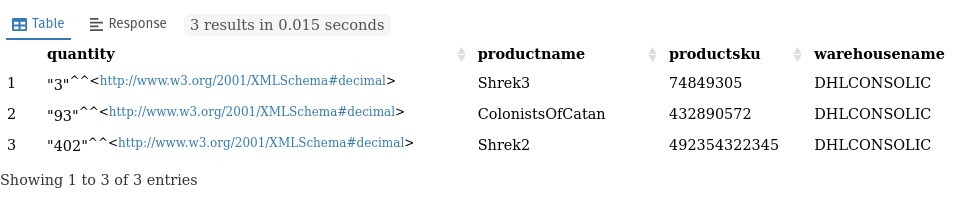
\includegraphics[scale=0.5]{OISreport-warehouse-query.png}
   \captionof{figure}{Query output}
\end{center}



\subsection{Costumers: Users with at least one complete address}
In a platform such as e-commerce, the admin should check and control customers' data. For handling this information, a query is available that gives the admin all the customers with at least one complete address. This can prevent errors such as a customer placing an order but doesn't have an address. This can also help the admin to manage the customers. This SPARQL query uses customers' information and their addresses. And it is also ordered by the first name of the customers. So the result contains the first name, last name, city address, city, and country of the customer.

\begin{lstlisting}[breaklines, frame=single]
PREFIX rdf: <http://www.w3.org/1999/02/22-rdf-syntax-ns#>
PREFIX rdfs: <http://www.w3.org/2000/01/rdf-schema#>
PREFIX ecommerce: http://data.ecommerce#
SELECT ?first_name ?last_name ?cityaddress ?city ?country WHERE{
	?customer ecommerce:first_name ?first_name;
			   ecommerce:last_name ?last_name;
			   ecommerce:Customer_email ?email.
	?address ecommerce:Customer_email ?email;
			ecommerce:Address_address ?cityaddress;
			ecommerce:Address_country ?city;
			ecommerce:Address_city ?country.
 } Order by ?first_name
\end{lstlisting}

\begin{center}
   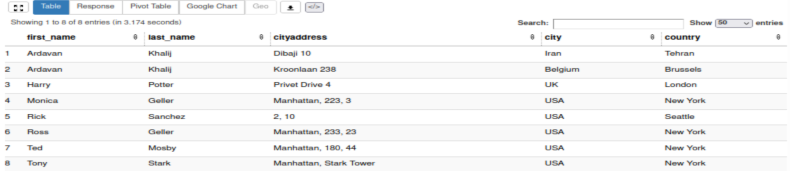
\includegraphics[scale=0.6]{OISreport-costumer-query.png}
   \captionof{figure}{Query output}
\end{center}

\subsection{Costumers: Customers with orders and the total amount of their orders}
In a platform such as e-commerce, the admin should be able to access all the order prices. This can help the admin to understand the income of the company. Customers also can access their orders to see the history of their purchases. This can always allow the customers to see what they have bought and re-order the products they want. This SPARQL uses the customers' information and the order information. And the result is also ordered by the total amount of each order. This can help the admin see which customers or customers with which home countries have the most considerable purchase amount per order. The result contains first name, last name, email, and the total amount of an order of the customer.

\begin{lstlisting}[breaklines, frame=single]
PREFIX rdf: <http://www.w3.org/1999/02/22-rdf-syntax-ns#>
PREFIX rdfs: <http://www.w3.org/2000/01/rdf-schema#>
PREFIX ecommerce: <http://data.ecommerce#>
SELECT ?first_name ?last_name ?email ?TotalAmount WHERE{
	?customer ecommerce:places_order ?order.
	?customer ecommerce:first_name ?first_name;
			  ecommerce:last_name ?last_name;
			  ecommerce:Customer_email ?email.
	?order ecommerce:orderAmount ?TotalAmount.
} ORDER BY ?TotalAmount
\end{lstlisting}

\begin{center}
   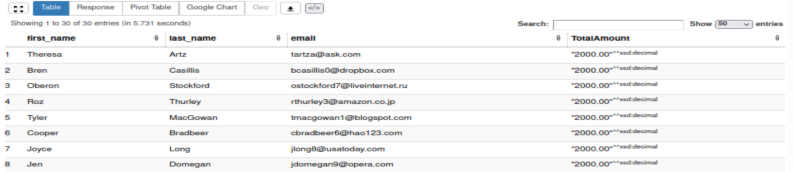
\includegraphics[scale=0.6]{OISreport-costumer-query2.png}
   \captionof{figure}{Query output}
\end{center}


\subsection{Supplier: Products with higher profit margin}
A platform such as e-commerce charges a percentage to a supplier for providing its service, in this case as an intermediary between its product and the customer. But the profit per product will depend on the price that the supplier sets. That is why it is necessary to know which products provide more profit to the platform to be able to make disguised biased advertising. As the price per product is not fixed, due to seasonal discounts that may exist, the average profit per product is disclosed, in this case the top 10 products with the highest profit margin. This decision may help the platform to have higher incomes. \\

\begin{lstlisting}[breaklines, frame=single]
PREFIX rdf: <http://www.w3.org/1999/02/22-rdf-syntax-ns#>
PREFIX rdfs: <http://www.w3.org/2000/01/rdf-schema#>
PREFIX ecommerce: <http://data.ecommerce#>
SELECT ?bce_company ?company ?product_code ?product_description (AVG(?price2) - AVG(?price1) AS ?profit)                              WHERE {
  ?supplier ecommerce:supplies ?supplies .
  ?supplier ecommerce:Supplierbce ?bce_company ;
           ecommerce:Supplier_companyName ?company .
  ?supplies ecommerce:supplies_has ?supply_stock .
  ?supply_stock ecommerce:has_contains ?product .
  ?supply_stock ecommerce:suppliesOrderPrice ?price1 .
  ?product ecommerce:sku ?product_code ;
           ecommerce:Product_description ?product_description ;
           ecommerce:price ?price2.
} GROUP BY ?bce_company ?company ?product_code ?product_description ORDER BY DESC(?profit) LIMIT 10
\end{lstlisting}

\begin{center}
   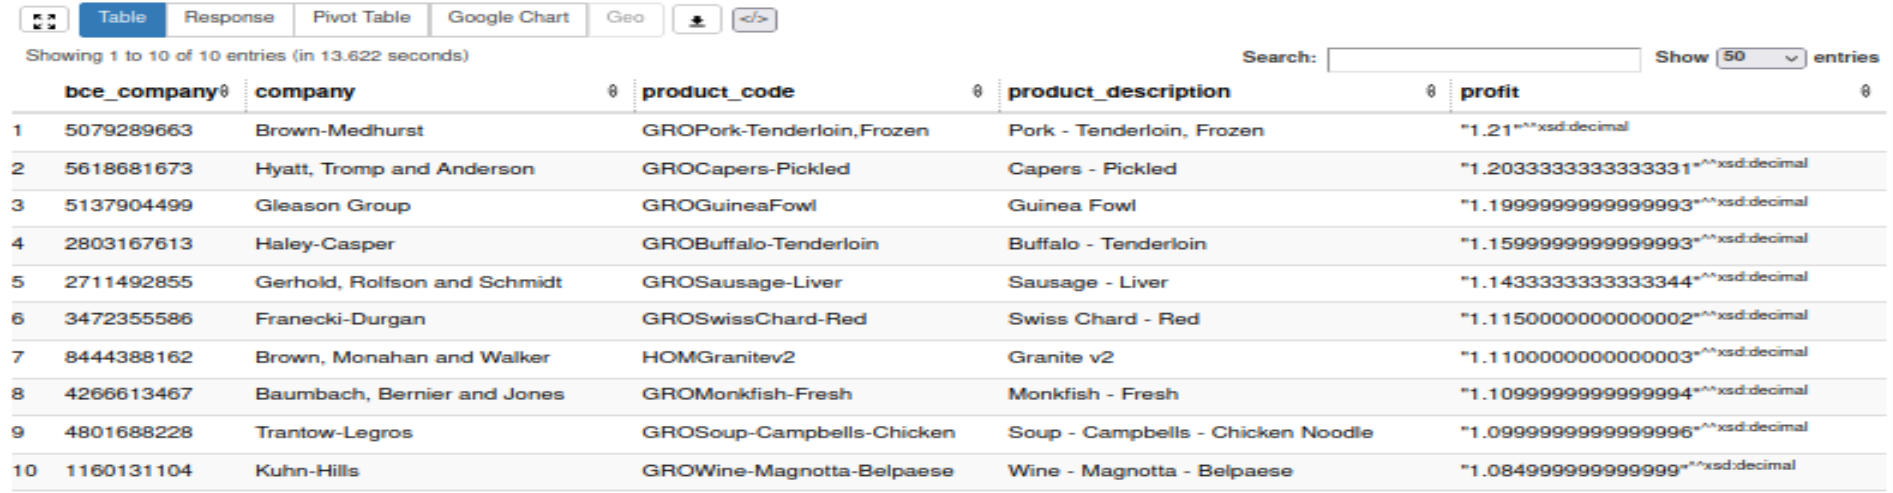
\includegraphics[scale=0.25]{OISreport-supplier-query.png}
   \captionof{figure}{Query output}
\end{center}



\subsection{Delivery services}





\section{Discussion}



\begin{thebibliography}{99}
\bibitem{OntopVK}
Guohui Xiao, Davide Lanti, Roman Kontchakov, Sarah Komla-Ebri, Elem Güzel-Kalayci, Linfang Ding, Julien Corman, Benjamin Cogrel, Diego Calvanese, and Elena Botoeva. (2020) \emph{The Virtual Knowledge Graph System Ontop}, International Semantic Web Conference.
\bibitem{OntopSPARQL}
Diego Calvanese, Benjamin Cogrel, Sarah Komla-Ebri, Roman Kontchakov, Davide Lanti, Martin Rezk, Mariano Rodriguez-Muro, and Guohui Xiao. (2017) \emph{Ontop: Answering SPARQL Queries over Relational Databases}, Semantic Web Journal 8.3, pp. 471–487.
\end{thebibliography}






\end{document}
